% !TEX root = ../../thesis.tex

\documentclass[../../thesis.tex]{subfiles}
 
\begin{document}

In this chapter, we experiment our solvers and discuss the results. 
We first talk about how we generated test instances to run our experiments and how 
those experiments were run.

\section{Instances generation}

To be able to make meaninful experiments, we need test data. Unfortunately, we were 
not able to be provided with real testing data. 
We had to generate data randomly with a series of parameters and probabilities passed 
to an instance generator. 

\section{Benchmark process}

\section{Constraint Programming}

\subsection{Heuristics}

\autoref{experiments:heuristic1} shows the objective ratio between the implemented custom \textit{Most Available} Heuristic and a standard 
\textit{First Fail} heuristic after the first solution. The two heuristics were tested on 72 instances of various sizes from small to big instances.
The performance profile shows a gain of about $2$ to $3.4$ for our custom heuristic.


\begin{figure}
  \centering
  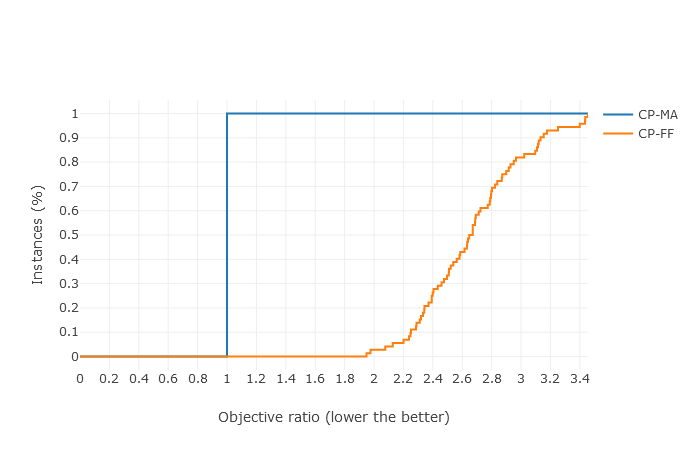
\includegraphics[scale=0.55]{experiments/heuristic.png}
  \caption{Most Available and First Fail heuristics [72 instances/first solution].}
  \label{experiments:heuristic1}
\end{figure}

\begin{figure}
  \centering
  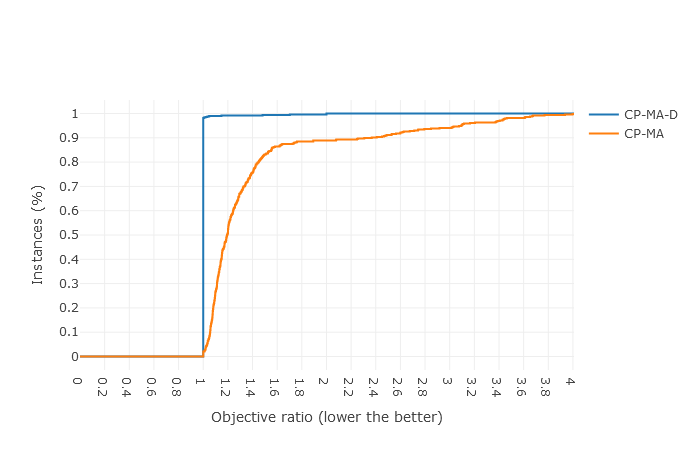
\includegraphics[scale=0.55]{experiments/static-dynamic-heuristic.png}
  \caption{Most Available: static and dynamic [486 instances/15s].}
  \label{experiments:heuristic2}
\end{figure}


\subsection{Large Neighborhood Search}


\section{Comparing solvers}

We now start by comparing different solvers together. \autoref{experiments:solvers:3} 
shows a performance profile generated from 216 instances of various sizes.
This benchmark was set to a time limit of 30s per instance. The baseline of this 
profile is the CP solver. We observe that the CP solver performs better than MIP in more than 80\% of instances.
However, we also tested the MIP solver by giving it a first solution obtained from CP, we can see that it slightly outperforms CP and MIP in 80\% of instances.

\begin{figure}
  \centering
  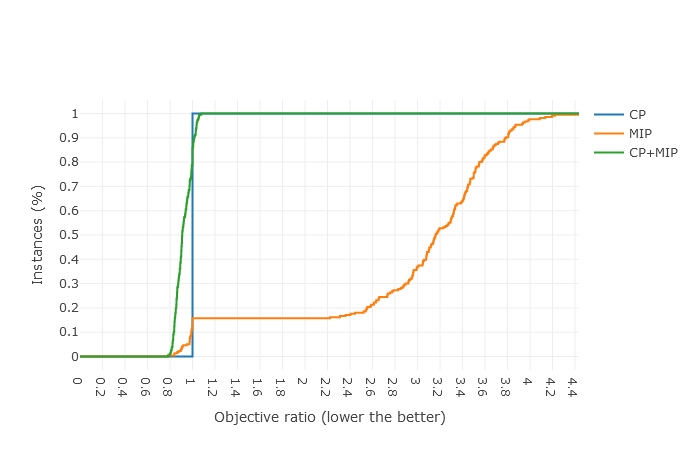
\includegraphics[scale=0.55]{experiments/solvers.png}
  \caption{CP, MIP and CP+MIP solvers [216 instances/30s].}
  \label{experiments:solvers:3}
\end{figure}


\begin{figure}
  \centering
  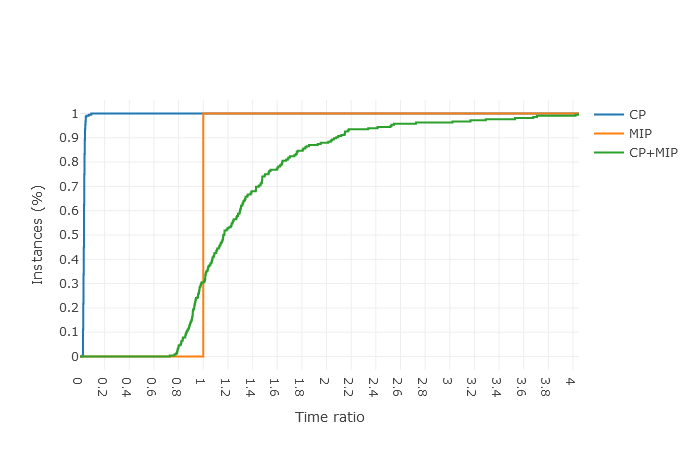
\includegraphics[scale=0.55]{experiments/time-first-sol.png}
  \caption{Time on first solution [216 instances/First solution].}
  \label{experiments:first-sol-time}
\end{figure}


\begin{figure}
  \centering
  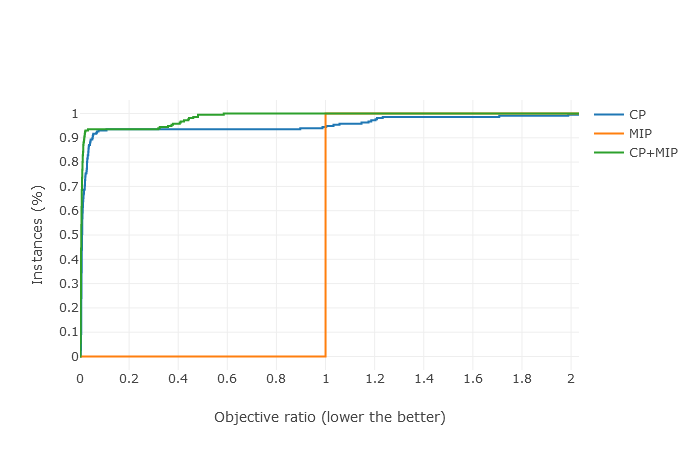
\includegraphics[scale=0.55]{experiments/obj-first-sol.png}
  \caption{Objective on first solution [216 instances/First solution].}
  \label{experiments:first-sol-obj}
\end{figure}




\end{document}

